\chapter{Análisis}

A lo largo de esta sección se irán analizando los requisitos para el desarrollo del proyecto. La aplicación cubre la gestión de usuarios, administradores de establecimiento, establecimientos, actividades, eventos, ofertas y reseñas. Además, se describirán los requisitos no funcionales del sistema para garantizar una experiencia de usuario óptima y del correcto funcionamiento de la aplicación.

\section{Requisitos Funcionales}

Los requisitos funcionales son una parte esencial del desarrollo de sistemas, ya que capturan el comportamiento previo del sistema. Este comportamiento se puede expresar como servicios, tareas o funciones que el sistema debe realizar. Los requisitos funcionales se centran en lo que el sistema hará, describiendo el comportamiento del sistema en
términos de las acciones específicas que debe llevar a  cabo para cumplir con las necesidades y expectativas del usuario final \cite{malan_bredemeyer} \cite{shah} \cite{sagar}.

A continuación se describirán los requisitos funcionales, divididos en apartados según su gestión principal. Esto permitirá una comprensión clara y detallada de los procesos y funcionalidades que la aplicación debe incluir para cumplir con sus objetivos y proporcionar una experiencia completa a sus usuarios.


\subsection{Gestión de Usuarios}

Este apartado describe las funcionalidades relativas a los usuarios. Al hablar de “Usuario” se referirá tanto a los usuarios genéricos del sistema como a un administrador de establecimiento. A continuación, se detallarán las funcionalidades para poder satisfacer las necesidades básicas de los usuarios:

\begin{table}[H]
    \centering
    \begin{tabular}{|c|p{10cm}|}
        \hline
        \multicolumn{2}{|c|}{\textbf{RF1 - Registro de Usuario}}                          \\
        \hline
        \textbf{Descripción}      & Permite a un nuevo usuario registrarse en el sistema. \\
        \hline
        \textbf{Datos de entrada} & Datos del usuario.                                    \\
        \hline
        \textbf{Datos de salida}  & Confirmación de registro exitoso.                     \\
        \hline
    \end{tabular}
    \caption{RF1 - Registro de Usuario}
\end{table}

\begin{table}[H]
    \centering
    \begin{tabular}{|c|p{10cm}|}
        \hline
        \multicolumn{2}{|c|}{\textbf{RF2 - Inicio de Sesión}}                                                                            \\
        \hline
        \textbf{Descripción}      & Permite a un usuario autenticarse e iniciar sesión en el sistema.                                    \\
        \hline
        \textbf{Datos de entrada} & Credenciales del usuario.                                                                            \\
        \hline
        \textbf{Datos de salida}  & Pantalla de inicio de usuario dependiendo si es usuario genérico o administrador de establecimiento. \\
        \hline
    \end{tabular}
    \caption{RF2 - Inicio de Sesión}
\end{table}

\begin{table}[H]
    \centering
    \begin{tabular}{|c|p{10cm}|}
        \hline
        \multicolumn{2}{|c|}{\textbf{RF3 - Consultar Usuario}}                                     \\
        \hline
        \textbf{Descripción}      & Permite ver la información del usuario que ha iniciado sesión. \\
        \hline
        \textbf{Datos de entrada} & Identificador del usuario.                                     \\
        \hline
        \textbf{Datos de salida}  & Datos del usuario.                                             \\
        \hline
    \end{tabular}
    \caption{RF3 - Consultar Usuario}
\end{table}

\begin{table}[H]
    \centering
    \begin{tabular}{|c|p{10cm}|}
        \hline
        \multicolumn{2}{|c|}{\textbf{RF4 - Modificar Usuario}}                                 \\
        \hline
        \textbf{Descripción}      & Permite actualizar los datos de un usuario en el sistema.  \\
        \hline
        \textbf{Datos de entrada} & Identificador del usuario, datos actualizados del usuario. \\
        \hline
        \textbf{Datos de salida}  & Confirmación de modificación exitosa.                      \\
        \hline
    \end{tabular}
    \caption{RF4 - Modificar Usuario}
\end{table}

\begin{table}[H]
    \centering
    \begin{tabular}{|c|p{10cm}|}
        \hline
        \multicolumn{2}{|c|}{\textbf{RF5 - Baja de Usuario}}                                               \\
        \hline
        \textbf{Descripción}      & Permite eliminar un usuario del sistema junto con sus datos asociados. \\
        \hline
        \textbf{Datos de entrada} & Identificador del usuario.                                             \\
        \hline
        \textbf{Datos de salida}  & Confirmación de baja exitosa.                                          \\
        \hline
    \end{tabular}
    \caption{RF5 - Baja de Usuario}
\end{table}

\begin{table}[H]
    \centering
    \begin{tabular}{|c|p{10cm}|}
        \hline
        \multicolumn{2}{|c|}{\textbf{RF6 - Seguir a Usuario}}                                                                     \\
        \hline
        \textbf{Descripción}      & Permite a un usuario seguir a otro usuario en el sistema, añadiéndolo a su lista de seguidos. \\
        \hline
        \textbf{Datos de entrada} & Identificador del usuario a seguir.                                                           \\
        \hline
        \textbf{Datos de salida}  & Confirmación de seguimiento de usuario, actualización de la lista de seguidos.                \\
        \hline
    \end{tabular}
    \caption{RF6 - Seguir a Usuario}
\end{table}

\begin{table}[H]
    \centering
    \begin{tabular}{|c|p{10cm}|}
        \hline
        \multicolumn{2}{|c|}{\textbf{RF7 - Dejar de Seguir a Usuario}}                                                                       \\
        \hline
        \textbf{Descripción}      & Permite a un usuario dejar de seguir a otro usuario en el sistema, eliminándolo de su lista de seguidos. \\
        \hline
        \textbf{Datos de entrada} & Identificador del usuario a dejar de seguir.                                                             \\
        \hline
        \textbf{Datos de salida}  & Confirmación de que se ha dejado de seguir a usuario, actualización de su lista de seguidos.             \\
        \hline
    \end{tabular}
    \caption{RF7 - Dejar de Seguir a Usuario}
\end{table}

\subsection{Gestión de Establecimientos}

Este apartado describe las funcionalidades relativas a los establecimientos, es decir, qué se puede hacer con ellos. A continuación, se detallarán las principales características y acciones disponibles para la gestión de los establecimientos dentro de la aplicación:

\begin{table}[H]
    \centering
    \begin{tabular}{|c|p{10cm}|}
        \hline
        \multicolumn{2}{|c|}{\textbf{RF8 - Crear Establecimiento}}                                                                                    \\
        \hline
        \textbf{Descripción}      & Permite a un administrador crear un nuevo establecimiento.                                                        \\
        \hline
        \textbf{Datos de entrada} & Datos del establecimiento.                                                                                        \\
        \hline
        \textbf{Datos de salida}  & Confirmación de la creación del establecimiento, actualización de la lista de establecimientos del administrador. \\
        \hline
    \end{tabular}
    \caption{RF8 - Crear Establecimiento}
\end{table}

\begin{table}[H]
    \centering
    \begin{tabular}{|c|p{10cm}|}
        \hline
        \multicolumn{2}{|c|}{\textbf{RF9 - Modificar Establecimiento}}                                         \\
        \hline
        \textbf{Descripción}      & Permite a un administrador actualizar los datos de un establecimiento.     \\
        \hline
        \textbf{Datos de entrada} & Identificador del establecimiento, datos actualizados del establecimiento. \\
        \hline
        \textbf{Datos de salida}  & Confirmación de modificación exitosa.                                      \\
        \hline
    \end{tabular}
    \caption{RF9 - Modificar Establecimiento}
\end{table}

\begin{table}[H]
    \centering
    \begin{tabular}{|c|p{10cm}|}
        \hline
        \multicolumn{2}{|c|}{\textbf{RF10 - Consultar Establecimiento}}                                                           \\
        \hline
        \textbf{Descripción}      & Permite a un usuario o administrador consultar los datos de un establecimiento en específico. \\
        \hline
        \textbf{Datos de entrada} & Identificador del establecimiento.                                                            \\
        \hline
        \textbf{Datos de salida}  & Datos del establecimiento.                                                                    \\
        \hline
    \end{tabular}
    \caption{RF10 - Consultar Establecimiento}
\end{table}

\begin{table}[H]
    \centering
    \begin{tabular}{|c|p{10cm}|}
        \hline
        \multicolumn{2}{|c|}{\textbf{RF11 - Eliminar Establecimiento}}                                                \\
        \hline
        \textbf{Descripción}      & Permite a un administrador eliminar un establecimiento.                           \\
        \hline
        \textbf{Datos de entrada} & Identificador del establecimiento.                                                \\
        \hline
        \textbf{Datos de salida}  & Confirmación de eliminación exitosa, actualización de la lista del administrador. \\
        \hline
    \end{tabular}
    \caption{RF11 - Eliminar Establecimiento}
\end{table}

\begin{table}[H]
    \centering
    \begin{tabular}{|c|p{10cm}|}
        \hline
        \multicolumn{2}{|c|}{\textbf{RF12 - Filtrar Establecimientos}}                                                        \\
        \hline
        \textbf{Descripción}      & Permite a un usuario poder filtrar los establecimientos según las preferencias indicadas. \\
        \hline
        \textbf{Datos de entrada} & Filtro aplicado.                                                                          \\
        \hline
        \textbf{Datos de salida}  & Establecimientos que cumplan con el filtro.                                               \\
        \hline
    \end{tabular}
    \caption{RF12 - Filtrar Establecimiento}
\end{table}

\subsection{Gestión de Eventos}

Este apartado describe la gestión de los eventos asociados a un establecimiento específico. Los eventos son importantes porque permiten a los establecimientos promocionar sus servicios, ayudando a los usuarios a decidir cuál se ajusta según sus necesidades. A continuación, se detallarán las principales acciones disponibles para la gestión de eventos:

\begin{table}[H]
    \centering
    \begin{tabular}{|c|p{10cm}|}
        \hline
        \multicolumn{2}{|c|}{\textbf{RF13 - Crear Evento}}                                                                                                       \\
        \hline
        \textbf{Descripción}      & Permite a un administrador crear un nuevo evento asociado a un establecimiento.                                              \\
        \hline
        \textbf{Datos de entrada} & Datos del evento                                                                                                             \\
        \hline
        \textbf{Datos de salida}  & Confirmación de creación del evento, actualización de la lista eventos del establecimiento en el cual se ha creado el evento \\
        \hline
    \end{tabular}
    \caption{RF13 - Crear Evento}
\end{table}

\begin{table}[H]
    \centering
    \begin{tabular}{|c|p{10cm}|}
        \hline
        \multicolumn{2}{|c|}{\textbf{RF14 - Modificar Evento}}                                                         \\
        \hline
        \textbf{Descripción}      & Permite a un administrador de establecimiento modificar un nuevo evento existente. \\
        \hline
        \textbf{Datos de entrada} & Identificador del evento, datos actualizados del evento.                           \\
        \hline
        \textbf{Datos de salida}  & Confirmación de modificación exitosa.                                              \\
        \hline
    \end{tabular}
    \caption{RF14 - Modificar Evento}
\end{table}

\begin{table}[H]
    \centering
    \begin{tabular}{|c|p{10cm}|}
        \hline
        \multicolumn{2}{|c|}{\textbf{RF15 - Consultar Evento}}                                                     \\
        \hline
        \textbf{Descripción}      & Permite a un usuario o administrador ver los datos de un evento en específico. \\
        \hline
        \textbf{Datos de entrada} & Identificador del evento.                                                      \\
        \hline
        \textbf{Datos de salida}  & Datos del evento.                                                              \\
        \hline
    \end{tabular}
    \caption{RF15 - Consultar Evento}
\end{table}

\begin{table}[H]
    \centering
    \begin{tabular}{|c|p{10cm}|}
        \hline
        \multicolumn{2}{|c|}{\textbf{RF16 - Eliminar Evento}}                                                                                              \\
        \hline
        \textbf{Descripción}      & Permite a un administrador eliminar un evento existente.                                                               \\
        \hline
        \textbf{Datos de entrada} & Identificador del evento.                                                                                              \\
        \hline
        \textbf{Datos de salida}  & Confirmación de eliminación exitosa, actualización de la lista de eventos del establecimiento que contenía ese evento. \\
        \hline
    \end{tabular}
    \caption{RF16 - Eliminar Evento}
\end{table}

\subsection{Gestión de Ofertas}

Este apartado describe la gestión de las ofertas asociadas a un establecimiento específico. Las ofertas son importantes porque permiten a los establecimientos promocionar sus servicios, ayudando a los usuarios a decidir cuál les conviene más entre los disponibles. A  continuación, se detallarán las principales acciones disponibles para la gestión de ofertas:

\begin{table}[H]
    \centering
    \begin{tabular}{|c|p{10cm}|}
        \hline
        \multicolumn{2}{|c|}{\textbf{RF17 - Crear Oferta}}                                                                                                         \\
        \hline
        \textbf{Descripción}      & Permiet a un administrador crear una nueva oferta asociada a un establecimiento.                                               \\
        \hline
        \textbf{Datos de entrada} & Datos de la oferta.                                                                                                            \\
        \hline
        \textbf{Datos de salida}  & Confirmación de creación exitosa, actualizacion de la lista de ofertas del establecimiento en el cual se ha creado esa oferta. \\
        \hline
    \end{tabular}
    \caption{RF17 - Crear Oferta}
\end{table}

\begin{table}[H]
    \centering
    \begin{tabular}{|c|p{10cm}|}
        \hline
        \multicolumn{2}{|c|}{\textbf{RF18 - Modificar Oferta}}                                   \\
        \hline
        \textbf{Descripción}      & Permite a un administrador modificar una oferta existente.   \\
        \hline
        \textbf{Datos de entrada} & Identificador de la oferta, datos actualizados de la oferta. \\
        \hline
        \textbf{Datos de salida}  & Confirmación de modificación exitosa.                        \\
        \hline
    \end{tabular}
    \caption{RF18 - Modificar Oferta}
\end{table}

\begin{table}[H]
    \centering
    \begin{tabular}{|c|p{10cm}|}
        \hline
        \multicolumn{2}{|c|}{\textbf{RF19 - Consultar Oferta}}                                                      \\
        \hline
        \textbf{Descripción}      & Permite a un usuario o administrador ver los datos de una oferta en específica. \\
        \hline
        \textbf{Datos de entrada} & Identificador de la oferta.                                                     \\
        \hline
        \textbf{Datos de salida}  & Datos de la oferta.                                                             \\
        \hline
    \end{tabular}
    \caption{RF19 - Consultar Oferta}
\end{table}

\begin{table}[H]
    \centering
    \begin{tabular}{|c|p{10cm}|}
        \hline
        \multicolumn{2}{|c|}{\textbf{RF20 - Eliminar Oferta}}                                                                                              \\
        \hline
        \textbf{Descripción}      & Permite a un administrador eliminar una oferta existente.                                                              \\
        \hline
        \textbf{Datos de entrada} & Identificador de la oferta.                                                                                            \\
        \hline
        \textbf{Datos de salida}  & Confirmación de eliminación exitosa, actualización de la lista de ofertas del establecimiento que contenía esa oferta. \\
        \hline
    \end{tabular}
    \caption{RF20 - Eliminar Oferta}
\end{table}

\subsection{Gestión de Actividades}

Este apartado describe la gestión de las actividades creadas por los usuarios para su grupo social cercano, con el fin de organizar y planificar salidas. A continuación, se detallan las principales acciones disponibles para la gestión de actividades:

\begin{table}[H]
    \centering
    \begin{tabular}{|c|p{10cm}|}
        \hline
        \multicolumn{2}{|c|}{\textbf{RF21 - Crear Actividad}}                                                                               \\
        \hline
        \textbf{Descripción}      & Permite a un usuario crear una nueva actividad.                                                         \\
        \hline
        \textbf{Datos de entrada} & Datos de la actividad.                                                                                  \\
        \hline
        \textbf{Datos de salida}  & Confirmación de creación de la actividad, actualización de la lista de actividades creadas del usuario. \\
        \hline
    \end{tabular}
    \caption{RF21 - Crear Actividad}
\end{table}

\begin{table}[H]
    \centering
    \begin{tabular}{|c|p{10cm}|}
        \hline
        \multicolumn{2}{|c|}{\textbf{RF22 - Modificar Actividad}}                                      \\
        \hline
        \textbf{Descripción}      & Permite a un usuario modificar una actividad creada.               \\
        \hline
        \textbf{Datos de entrada} & Identificador de la actividad, datos actualizados de la actividad. \\
        \hline
        \textbf{Datos de salida}  & Confirmación de modificación exitosa.                              \\
        \hline
    \end{tabular}
    \caption{RF2 - Modificar Actividad}
\end{table}

\begin{table}[H]
    \centering
    \begin{tabular}{|c|p{10cm}|}
        \hline
        \multicolumn{2}{|c|}{\textbf{RF23 - Consultar Actividad}}                                                              \\
        \hline
        \textbf{Descripción}      & Permite a un usuario poder consultar los datos de una actividad en la cual este participe. \\
        \hline
        \textbf{Datos de entrada} & Identificador de la actividad.                                                             \\
        \hline
        \textbf{Datos de salida}  & Datos de la actividad.                                                                     \\
        \hline
    \end{tabular}
    \caption{RF23 - Consultar Actividad}
\end{table}

\begin{table}[H]
    \centering
    \begin{tabular}{|c|p{10cm}|}
        \hline
        \multicolumn{2}{|c|}{\textbf{RF24 - Eliminar Actividad}}                                                                       \\
        \hline
        \textbf{Descripción}      & Permite a un usuario eliminar una actividad creada.                                                \\
        \hline
        \textbf{Datos de entrada} & Identificador de la actividad.                                                                     \\
        \hline
        \textbf{Datos de salida}  & Confirmación de eliminación exitosa, actualización de la lista de actividades creadas del usuario. \\
        \hline
    \end{tabular}
    \caption{RF24 - Eliminar Actividad}
\end{table}

\begin{table}[H]
    \centering
    \begin{tabular}{|c|p{10cm}|}
        \hline
        \multicolumn{2}{|c|}{\textbf{RF25 - Invitar Usuario a Actividad}}                                                                                   \\
        \hline
        \textbf{Descripción}      & Permite a un usuario invitar a otros usuarios a participar en una actividad.                                            \\
        \hline
        \textbf{Datos de entrada} & Identificador del usuario a invitar.                                                                                    \\
        \hline
        \textbf{Datos de salida}  & Confirmación de adición de un nuevo usuario a la actividad, actualización de la lista de participantes de la actividad. \\
        \hline
    \end{tabular}
    \caption{RF25 - Invitar Usuario a Actividad}
\end{table}

\subsection{Gestión de Reseñas}

Este apartado describe la gestión de las reseñas a un establecimiento. Las reseñas son cruciales para mostrar a los usuarios los establecimientos según las evaluaciones y comentarios de otros clientes. Además, son importantes para los administradores de establecimientos, ya que pueden utilizar el feedback para mejorar sus servicios. A continuación, se detallan las principales acciones para la gestión de las reseñas:

\begin{table}[H]
    \centering
    \begin{tabular}{|c|p{10cm}|}
        \hline
        \multicolumn{2}{|c|}{\textbf{RF26 - Crear Reseña}}                                                                                                                                                 \\
        \hline
        \textbf{Descripción}      & Permite a un usuario dejar reseñas a un establecimiento.                                                                                                               \\
        \hline
        \textbf{Datos de entrada} & dentificador del establecimiento, datos de la reseña.                                                                                                                  \\
        \hline
        \textbf{Datos de salida}  & Confirmación de que la reseña ha sido publicada, actualización de la lista de reseñas del establecimiento, actualización de las listas de reseñas creadas del usuario. \\
        \hline
    \end{tabular}
    \caption{RF26 - Crear Reseña}
\end{table}

\begin{table}[H]
    \centering
    \begin{tabular}{|c|p{10cm}|}
        \hline
        \multicolumn{2}{|c|}{\textbf{RF27 - Consultar Reseña}}                                                             \\
        \hline
        \textbf{Descripción}      & Permite a un usuario o administrador ver las reseñas de un establecimiento específico. \\
        \hline
        \textbf{Datos de entrada} & Identificador del establecimiento.                                                     \\
        \hline
        \textbf{Datos de salida}  & Reseñas del establecimiento.                                                           \\
        \hline
    \end{tabular}
    \caption{RF27 - Consultar Reseña}
\end{table}

\section{Requisitos No Funcionales}

Los requisitos no funcionales son aquellos que especifican los criterios que pueden ser utilizados para juzgar el funcionamiento de un sistema, en lugar de describir los comportamientos específicos. A diferencia de los requisitos funcionales, que detallan lo que el sistema debe hacer, los requisitos no funcionales definen cómo debe ser el sistema en términos de calidad y restricciones operativas, asegurando que el sistema cumpla con los estándares de calidad esperados \cite{glinz} \cite{chung} \cite{gross}.

\begin{table}[H]
    \centering
    \begin{tabular}{|c|p{10cm}|}
        \hline
        \multicolumn{2}{|c|}{\textbf{RNF1 - Usabilidad}}                                       \\
        \hline
        \textbf{Descripción} & La aplicación será intuitiva y fácil de usar para los usuarios. \\
        \hline
        \textbf{Criterios}   & Interfaz de usuario sencilla e intuitiva.                       \\
        \hline
    \end{tabular}
    \caption{RNF1 - Usabilidad}
\end{table}

\begin{table}[H]
    \centering
    \begin{tabular}{|c|p{10cm}|}
        \hline
        \multicolumn{2}{|c|}{\textbf{RNF2 - Rendimiento}}                                             \\
        \hline
        \textbf{Descripción} & La aplicación deberá responder rápidamente a las consultas realizadas. \\
        \hline
        \textbf{Criterios}   & Tiempos de respuestas rápidos para las peticiones realizadas.          \\
        \hline
    \end{tabular}
    \caption{RNF2 - Rendimiento}
\end{table}

\begin{table}[H]
    \centering
    \begin{tabular}{|c|p{10cm}|}
        \hline
        \multicolumn{2}{|c|}{\textbf{RNF3 - Seguridad}}                                                                              \\
        \hline
        \textbf{Descripción} & La aplicación protegerá la información sensible relacionada con los datos personales de los usuarios. \\
        \hline
        \textbf{Criterios}   & Los datos sensibles de los usuarios solo podrán ser consultados por ellos mismos.                     \\
        \hline
    \end{tabular}
    \caption{RNF3 - Seguridad}
\end{table}

\begin{table}[H]
    \centering
    \begin{tabular}{|c|p{10cm}|}
        \hline
        \multicolumn{2}{|c|}{\textbf{RNF4 - Compatibilidad}}                                                                                                 \\
        \hline
        \textbf{Descripción} & La aplicación funcionará correctamente independientemente del dispositivo móvil utilizado siempre y cuando sea un smartphone. \\
        \hline
        \textbf{Criterios}   & El diseño del frontend en React Native permite poder desplegar el archivo APK para Android y el archivo para iOS.             \\
        \hline
    \end{tabular}
    \caption{RNF4 - Compatibilidad}
\end{table}

\begin{table}[H]
    \centering
    \begin{tabular}{|c|p{10cm}|}
        \hline
        \multicolumn{2}{|c|}{\textbf{RNF5 - Escalabilidad}}                                                                                  \\
        \hline
        \textbf{Descripción} & La aplicación debe ser capaz de escalar y manejar el aumento de la carga manteniendo el nivel de rendimiento. \\
        \hline
        \textbf{Criterios}   & El sistema permite el crecimiento de carga según aumente el número de usuarios gracias a su arquitectura.     \\
        \hline
    \end{tabular}
    \caption{RNF5 - Escalabilidad}
\end{table}

\begin{table}[H]
    \centering
    \begin{tabular}{|c|p{10cm}|}
        \hline
        \multicolumn{2}{|c|}{\textbf{RNF6 - Mantenibilidad}}                                                                                                                                                     \\
        \hline
        \textbf{Descripción} & La aplicación debe poder proveer actualizaciones y mantenimiento regulable para su continuo desarrollo.                                                                           \\
        \hline
        \textbf{Criterios}   & La documentación se realizará de una forma clara permitiendo el entendimiento del código y podiendo realizar actualizaciones para el beneficio de la experiencia de los usuarios. \\
        \hline
    \end{tabular}
    \caption{RNF6 - Mantenibilidad}
\end{table}

\section{Modelos de Caso de Uso}

Los modelos de caso de uso son representaciones gráficas que describen cómo los usuarios interactúan con el sistema para lograr un objetivo específico. Estos modelos se utilizan para capturar y definir los requisitos funcionales del sistema., identificando las diferentes formas en que los usuarios pueden utilizar el sistema y las respuestas del sistema a estas interacciones. Los modelos de casos de uso ayudan a comunicar claramente las funcionalidades esperadas del sistema a todas las partes interesadas, asegurando que todos tengan una comprensión común de los requerimientos \cite{ibm}. 

\subsection{Actores del Sistema}

La interacción de la aplicación se basa en dos tipos de actores: usuarios genéricos y administradores de establecimiento. Es importante destacar que el acceso a la aplicación está restringida a usuarios registrados, ya que se busca asegurar que cada interacción dentro del sistema se realice de una manera personalizada.

\begin{enumerate}
    \item \textbf{Usuario Genérico:} Los usuarios genéricos son los clientes de la aplicación, aquellos para los cuales está destinado su uso. Pueden consultar establecimientos según las preferencias indicadas, ver las ofertas y eventos disponibles, y crear actividades sociales. Estas funcionalidades permiten a los usuarios personalizar su experiencia y aprovechar al máximo los servicios ofrecidos por la aplicación.

    \item \textbf{Administrador de Establecimiento:} Los administradores de establecimientos interactúan con la aplicación para la creación, administración y promoción de sus establecimientos. Esto incluye la creación de ofertas y eventos, así como la gestión general de la información del establecimiento. Estas funcionalidades permiten a los administradores optimizar la visibilidad y el atractivo de sus establecimientos dentro de la aplicación.
\end{enumerate}

\subsection{Escenarios de Casos de Uso}

\begin{table}[h]
    \centering
    \begin{tabular}{|c|p{10cm}|}
        \hline
        \multicolumn{2}{|c|}{\textbf{CU1 - Registrar Usuario}}                               \\
        \hline
        \textbf{Actores}         & Usuario Genérico y Administrador de Establecimiento.      \\
        \hline
        \textbf{Precondiciones}  & El actor no debe estar registrado en el sistema.          \\
        \hline
        \textbf{Postcondiciones} & El actor está registrado en el sistema.                   \\
        \hline
        \textbf{Flujo principal} & \begin{enumerate}
                                       \item El actor accede a la pantalla de registro.
                                       \item El actor ingresa sus datos.
                                       \item El sistema valida sus datos.
                                       \item El sistema registra al actor y confirma su registro.
                                   \end{enumerate} \\
        \hline
    \end{tabular}
    \caption{CU-1 Registrar Usuario}
\end{table}

\begin{table}[h]
    \centering
    \begin{tabular}{|c|p{10cm}|}
        \hline
        \multicolumn{2}{|c|}{\textbf{CU2 - Autenticar Usuario}}                                             \\
        \hline
        \textbf{Actores}         & Usuario Genérico y Administrador de Establecimiento                      \\
        \hline
        \textbf{Precondiciones}  & El actor debe estar registrado en el sistema                             \\
        \hline
        \textbf{Postcondiciones} & El usuario está autenticado en el sistema                                \\
        \hline
        \textbf{Flujo principal} & \begin{enumerate}
                                       \item El usuario accede a la pantalla de inicio de sesión.
                                       \item El usuario ingresa sus credenciales
                                       \item El sistema valida sus credenciales
                                       \item El sistema permite el acceso al usuario y confirma la autenticación
                                   \end{enumerate} \\
        \hline
    \end{tabular}
    \caption{CU2 - Autenticar Usuario }
\end{table}

\begin{table}[h]
    \centering
    \begin{tabular}{|c|p{10cm}|}
        \hline
        \multicolumn{2}{|c|}{\textbf{CU3 - Gestionar Usuario}}                         \\
        \hline
        \textbf{Actores}         & Usuario Genérico y Administrador de Establecimiento \\
        \hline
        \textbf{Precondiciones}  & El actor debe haber iniciado sesión en el sistema   \\
        \hline
        \textbf{Postcondiciones} & Los datos del usuario son gestionados               \\
        \hline
        \textbf{Flujo principal} & \begin{enumerate}
                                       \item El usuario accede a la pantalla de su perfil
                                       \item El usuario puede elegir entre:
                                             \begin{enumerate}
                      \item Consultar sus datos (Consultar Datos de Usuario)
                      \item Modificar sus datos (Modificar Usuario)
                      \item Eliminar su cuenta (Baja de Usuario)
                  \end{enumerate}
                                       \item El sistema valida y confirma sus acciones
                                   \end{enumerate}   \\
        \hline
    \end{tabular}
    \caption{CU3 - Gestionar Usuario }
\end{table}

\begin{table}[h]
    \centering
    \begin{tabular}{|c|p{10cm}|}
        \hline
        \multicolumn{2}{|c|}{\textbf{CU4 - Consultar Establecimiento}}                                \\
        \hline
        \textbf{Actores}         & Usuario Genérico y Administrador de Establecimiento                \\
        \hline
        \textbf{Precondiciones}  & El actor debe haber iniciado sesión en el sistema                  \\
        \hline
        \textbf{Postcondiciones} & Se mostrarán los datos de el establecimiento consultado            \\
        \hline
        \textbf{Flujo principal} & \begin{enumerate}
                                       \item El actor accede a la pantalla principal del sistema
                                       \item El actor navega hasta el establecimiento de interés
                                       \item El actor selecciona el establecimiento
                                       \item El sistema muestra los datos del establecimiento seleccionado
                                   \end{enumerate} \\
        \hline
    \end{tabular}
    \caption{CU4 - Consultar Establecimiento}
\end{table}

\begin{table}[h]
    \centering
    \begin{tabular}{|c|p{10cm}|}
        \hline
        \multicolumn{2}{|c|}{\textbf{CU5 - Consultar Reseñas}}                                                   \\
        \hline
        \textbf{Actores}         & Usuario Genérico y Administrador de Establecimiento                           \\
        \hline
        \textbf{Precondiciones}  & El actor debe haber iniciado sesión en el sistema                             \\
        \hline
        \textbf{Postcondiciones} & Se mostrarán los datos de las reseñas asociadas al establecimiento consultado \\
        \hline
        \textbf{Flujo principal} & \begin{enumerate}
                                       \item El actor accede a la pantalla principal del sistema
                                       \item El actor navega hasta el establecimiento de interés
                                       \item El actor selecciona el establecimiento
                                       \item El sistema muestra las reseñas asociadas a ese establecimiento
                                   \end{enumerate}           \\
        \hline
    \end{tabular}
    \caption{CU5 - Consultar Reseñas }
\end{table}

\begin{table}[h]
    \centering
    \begin{tabular}{|c|p{10cm}|}
        \hline
        \multicolumn{2}{|c|}{\textbf{CU6 - }}                                                               \\
        \hline
        \textbf{Actores}         & Usuario Genérico y Administrador de Establecimiento                      \\
        \hline
        \textbf{Precondiciones}  & El actor debe haber iniciado sesión en el sistema                        \\
        \hline
        \textbf{Postcondiciones} & Se mostrarán los datos del evento asociado al establecimiento consultado \\
        \hline
        \textbf{Flujo principal} & \begin{enumerate}
                                       \item El actor accede a la pantalla principal del sistema
                                       \item El actor navega hasta el establecimiento de interés
                                       \item El actor selecciona el establecimiento
                                       \item El actor selecciona un evento dentro de ese establecimiento
                                       \item El sistema muestra los datos del evento seleccionado.
                                   \end{enumerate}         \\
        \hline
    \end{tabular}
    \caption{CU6 - Consultar Eventos }
\end{table}

\begin{table}[h]
    \centering
    \begin{tabular}{|c|p{10cm}|}
        \hline
        \multicolumn{2}{|c|}{\textbf{CU7 - Consultar Ofertas}}                                       \\
        \hline
        \textbf{Actores}         & Usuario Genérico y Administrador de Establecimiento               \\
        \hline
        \textbf{Precondiciones}  & El actor debe haber iniciado sesión en el sistema                 \\
        \hline
        \textbf{Postcondiciones} &                                                                   \\
        \hline
        \textbf{Flujo principal} & \begin{enumerate}
                                       \item El actor accede a la pantalla principal del sistema
                                       \item El actor navega hasta el establecimiento de interés
                                       \item El actor selecciona el establecimiento
                                       \item El actor selecciona una oferta dentro de ese establecimiento
                                       \item El sistema muestra los datos de la oferta seleccionada
                                   \end{enumerate} \\
        \hline
    \end{tabular}
    \caption{CU7 - Consultar Ofertas }
\end{table}

\begin{table}[h]
    \centering
    \begin{tabular}{|c|p{10cm}|}
        \hline
        \multicolumn{2}{|c|}{\textbf{CU8 - Crear Establecimiento }}                                                                          \\
        \hline
        \textbf{Actores}         & Administrador de Establecimiento                                                                          \\
        \hline
        \textbf{Precondiciones}  & El administrador de establecimiento debe haber iniciado sesión en el sistema                              \\
        \hline
        \textbf{Postcondiciones} & Confirmación de creación de establecimiento, se actualiza la lista de establecimientos del administrador. \\
        \hline
        \textbf{Flujo principal} & \begin{enumerate}
                                       \item El administrador accede a su página principal.
                                       \item El administrador selecciona la opción de Crear Establecimiento.
                                       \item El administrador proporciona los datos del nuevo establecimiento.
                                       \item El sistema valida los datos ingresados.
                                       \item El sistema registra y confirma el nuevo establecimiento.
                                   \end{enumerate}                                    \\
        \hline
    \end{tabular}
    \caption{CU8 - Crear Establecimiento }
\end{table}

\begin{table}[h]
    \centering
    \begin{tabular}{|c|p{10cm}|}
        \hline
        \multicolumn{2}{|c|}{\textbf{CU9 - Gestionar Establecimiento}}                                              \\
        \hline
        \textbf{Actores}         & Administrador de Establecimiento                                                 \\
        \hline
        \textbf{Precondiciones}  & El administrador de establecimiento debe haber iniciado sesión en el sistema     \\
        \hline
        \textbf{Postcondiciones} & Los datos del establecimiento han sido adecuadamente gestionados                 \\
        \hline
        \textbf{Flujo principal} & \begin{enumerate}
                                       \item El administrador accede a su página principal.
                                       \item El administrador selecciona un establecimiento entre los que este gestiona.
                                       \item El administrador puede elegir entre:
                                             \begin{enumerate}
                      \item Modificar un establecimiento (Modificar Establecimiento)
                      \item Eliminar un Establecimiento (Eliminar Establecimiento)
                  \end{enumerate}
                                       \item El sistema valida y confirma las acciones
                                   \end{enumerate} \\
        \hline
    \end{tabular}
    \caption{CU9 - Gestionar Establecimiento }
\end{table}

\begin{table}[h]
    \centering
    \begin{tabular}{|c|p{10cm}|}
        \hline
        \multicolumn{2}{|c|}{\textbf{CU10 - Crear Evento}}                                                                                               \\
        \hline
        \textbf{Actores}         & Administrador de Establecimiento                                                                                      \\
        \hline
        \textbf{Precondiciones}  & El administrador de establecimiento debe haber iniciado sesión en el sistema                                          \\
        \hline
        \textbf{Postcondiciones} & Confirmación de creación de evento, se actualiza la lista de eventos del establecimiento.                             \\
        \hline
        \textbf{Flujo principal} & \begin{enumerate}
                                       \item El administrador accede a su página principal
                                       \item El administrador selecciona un establecimiento entre los que este gestiona.
                                       \item El administrador selecciona la opción de Crear Evento simbolizada con el signo + al lado de la etiqueta Eventos.
                                       \item El administrador proporciona los datos del nuevo evento.
                                       \item El sistema valida los datos ingresados.
                                       \item El sistema registra y confirma el nuevo evento
                                   \end{enumerate} \\
        \hline
    \end{tabular}
    \caption{CU10 - Crear Evento }
\end{table}

\begin{table}[h]
    \centering
    \begin{tabular}{|c|p{10cm}|}
        \hline
        \multicolumn{2}{|c|}{\textbf{CU11 - Gestionar Evento}}                                                         \\
        \hline
        \textbf{Actores}         & Administrador de Establecimiento                                                    \\
        \hline
        \textbf{Precondiciones}  & El administrador de establecimiento debe haber iniciado sesión en el sistema        \\
        \hline
        \textbf{Postcondiciones} & Los datos del evento han sido adecuadamente gestionados                             \\
        \hline
        \textbf{Flujo principal} & \begin{enumerate}
                                       \item El administrador accede a su página principal.
                                       \item El administrador selecciona un establecimiento entre los que este gestiona.
                                       \item El administrador selecciona un evento de los asociados a este establecimiento.
                                       \item El administrador puede elegir entre:
                                             \begin{enumerate}
                      \item Modificar un evento (Modificar Evento)
                      \item Eliminar un evento (Eliminar Evento)
                  \end{enumerate}
                                       \item El sistema valida y confirma las acciones

                                   \end{enumerate} \\
        \hline
    \end{tabular}
    \caption{CU11 - Gestionar Evento }
\end{table}

\begin{table}[h]
    \centering
    \begin{tabular}{|c|p{10cm}|}
        \hline
        \multicolumn{2}{|c|}{\textbf{CU12 - Crear Oferta}}                                                                                               \\
        \hline
        \textbf{Actores}         & Administrador de Establecimiento                                                                                      \\
        \hline
        \textbf{Precondiciones}  & El administrador de establecimiento debe haber iniciado sesión en el sistema                                          \\
        \hline
        \textbf{Postcondiciones} & Confirmación de creación de oferta, se actualiza la lista de ofertas del establecimiento.                             \\
        \hline
        \textbf{Flujo principal} & \begin{enumerate}
                                       \item El administrador accede a su página principal
                                       \item El administrador selecciona un establecimiento entre los que este gestiona.
                                       \item El administrador selecciona la opción de Crear Oferta simbolizada con el signo + al lado de la etiqueta Ofertas.
                                       \item El administrador proporciona los datos de la nueva oferta.
                                       \item El sistema valida los datos ingresados.
                                       \item El sistema registra y confirma la nueva oferta
                                   \end{enumerate} \\
        \hline
    \end{tabular}
    \caption{CU12 - Crear Oferta }
\end{table}

\begin{table}[h]
    \centering
    \begin{tabular}{|c|p{10cm}|}
        \hline
        \multicolumn{2}{|c|}{\textbf{CU13 - Gestionar Oferta}}                                                          \\
        \hline
        \textbf{Actores}         & Administrador de Establecimiento                                                     \\
        \hline
        \textbf{Precondiciones}  & El administrador de establecimiento debe haber iniciado sesión en el sistema         \\
        \hline
        \textbf{Postcondiciones} & Los datos de la oferta han sido adecuadamente gestionados                            \\
        \hline
        \textbf{Flujo principal} & \begin{enumerate}
                                       \item El administrador accede a su página principal.
                                       \item El administrador selecciona un establecimiento entre los que este gestiona.
                                       \item El administrador selecciona una oferta de las asociadas a este establecimiento.
                                       \item El administrador puede elegir entre:
                                             \begin{enumerate}
                      \item Modificar una oferta(Modificar Oferta)
                      \item Eliminar una oferta(Eliminar Oferta)
                  \end{enumerate}
                                       \item El sistema valida y confirma las acciones
                                   \end{enumerate} \\
        \hline
    \end{tabular}
    \caption{CU13 - Gestionar Oferta }
\end{table}

\begin{table}[h]
    \centering
    \begin{tabular}{|c|p{10cm}|}
        \hline
        \multicolumn{2}{|c|}{\textbf{CU14 - Crear Actividad}}                                                                                                          \\
        \hline
        \textbf{Actores}         & Usuario Genérico                                                                                                                    \\
        \hline
        \textbf{Precondiciones}  & El usuario debe haber iniciado sesión en el sistema                                                                                 \\
        \hline
        \textbf{Postcondiciones} & Confirmación de creación de actividad, se actualiza la lista de actividades creadas del usuario.                                    \\
        \hline
        \textbf{Flujo principal} & \begin{enumerate}
                                       \item El usuario accede a su página principal.
                                       \item El usuario selecciona la opción de \textbf{Crear Actividad} simbolizada con el signo \textbf{+} en el footer de la aplicación.
                                       \item El usuario proporciona los datos de la nueva actividad.
                                       \item El sistema valida los datos ingresados.
                                       \item El sistema confirma y registra la nueva actividad.
                                   \end{enumerate} \\
        \hline
    \end{tabular}
    \caption{CU14 - Crear Actividad }
\end{table}

\begin{table}[h]
    \centering
    \begin{tabular}{|c|p{10cm}|}
        \hline
        \multicolumn{2}{|c|}{\textbf{CU15 - Gestionar Actividad}}                              \\
        \hline
        \textbf{Actores}         & Usuario Genérico                                            \\
        \hline
        \textbf{Precondiciones}  & El usuario debe haber iniciado sesión en el sistema         \\
        \hline
        \textbf{Postcondiciones} & Los datos de la actividad han sido correctamente gestionado \\
        \hline
        \textbf{Flujo principal} & \begin{enumerate}
                                       \item El usuario accede a su página principal.
                                       \item El usuario navega hasta una actividad y la selecciona.
                                       \item El usuario puede elegir entre:
                                             \begin{enumerate}
                      \item Modificar una actividad(Modificar Actividad)
                      \item Eliminar una actividad(Eliminar Actividad)
                  \end{enumerate}
                                       \item El sistema valida y confirma las acciones
                                   \end{enumerate} \\
        \hline
    \end{tabular}
    \caption{CU15 - Gestionar Actividad }
\end{table}

\begin{table}[h]
    \centering
    \begin{tabular}{|c|p{10cm}|}
        \hline
        \multicolumn{2}{|c|}{\textbf{CU16 - Crear Reseña}}                                                                                                                                \\
        \hline
        \textbf{Actores}         & Usuario Genérico                                                                                                                                       \\
        \hline
        \textbf{Precondiciones}  & El usuario debe haber iniciado sesión en el sistema                                                                                                    \\
        \hline
        \textbf{Postcondiciones} & Confirmación de creación de reseña, se actualiza la lista de reseñas creadas por parte del usuario y se actualiza la lista reseñas del establecimiento \\
        \hline
        \textbf{Flujo principal} & \begin{enumerate}
                                       \item El usuario accede a su página principal.
                                       \item El usuario navega hasta un establecimiento y lo selecciona
                                       \item El usuario selecciona la opción de Crear Reseña simbolizada con el signo + al final de la pantalla del establecimiento.
                                       \item El usuario rellena la reseña asignándole una calificación al establecimiento.
                                       \item El sistema valida los datos proporcionados para la creación de la reseña .
                                       \item El sistema confirma y registra la nueva reseña
                                   \end{enumerate}                           \\
        \hline
    \end{tabular}
    \caption{CU16 - Crear Reseña }
\end{table}

\begin{table}[h]
    \centering
    \begin{tabular}{|c|p{10cm}|}
        \hline
        \multicolumn{2}{|c|}{\textbf{CU17 - Filtrar Establecimientos}}                                                                \\
        \hline
        \textbf{Actores}         & Usuario Genérico                                                                                   \\
        \hline
        \textbf{Precondiciones}  & El usuario debe haber iniciado sesión en el sistema                                                \\
        \hline
        \textbf{Postcondiciones} & Se mostrarán los establecimientos que cumplan con el filtro seleciconado por el usuario            \\
        \hline
        \textbf{Flujo principal} & \begin{enumerate}
                                       \item El usuario accede a su página principal.
                                       \item El usuario selecciona las preferencias.
                                       \item El sistema valida las preferencias y muestra los establecimientos que cumplan con ese filtro.
                                   \end{enumerate} \\
        \hline
    \end{tabular}
    \caption{CU17 - Filtrar Establecimientos }
\end{table}

\clearpage
\thispagestyle{empty}
\begin{figure}[H]
    \centering
    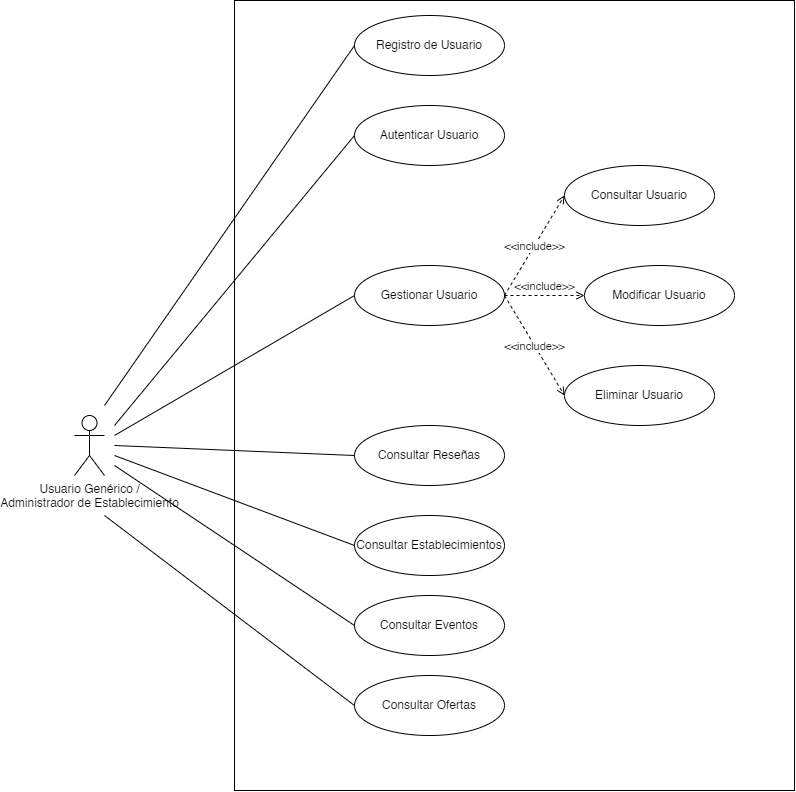
\includegraphics[width=\textwidth,height=\textheight,keepaspectratio]{imagenes/CasoDeUsoComun.jpg}
    \caption{Caso de Uso con Actores Comunes}
    \label{fig:CasoDeUsoComun}
\end{figure}

\clearpage
\thispagestyle{empty}
\begin{figure}[H]
    \centering
    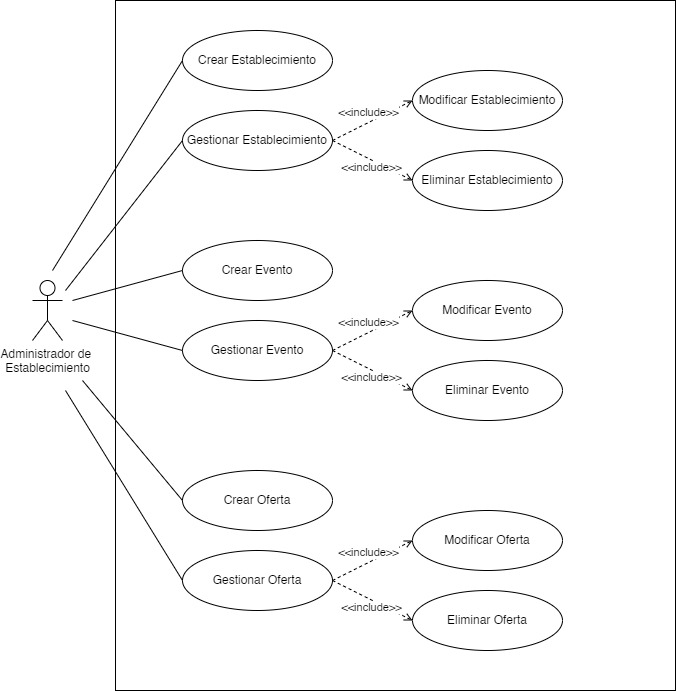
\includegraphics[width=\textwidth,height=\textheight,keepaspectratio]{imagenes/CasoDeUsoAdministrador.jpg}
    \caption{Caso de Uso con Administrador de Establecimiento}
    \label{fig:CasosDeUsoAdmin}
\end{figure}

\clearpage
\thispagestyle{empty}
\begin{figure}[H]
    \centering
    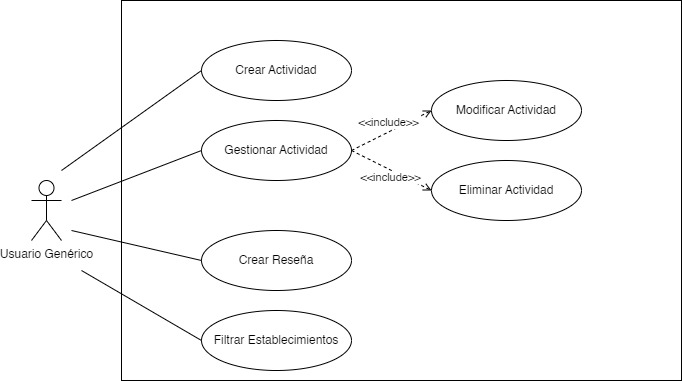
\includegraphics[width=\textwidth,height=\textheight,keepaspectratio]{imagenes/CasoDeUsoUsuario.jpg}
    \caption{Caso de Uso con Usuario Genérico}
    \label{fig:CasosDeUsoUser}
\end{figure}

